% Template taken with permission from Richard Hu
% Modified by Rahul Shah
% Last Updated: 2021-04-17 21:19

\documentclass[11pt]{article}
\usepackage{header}
\usepackage{mathrsfs}
\usepackage{mdframed}
\usepackage{pdfpages}
\usepackage{titlesec}

\newmdenv[%
    leftmargin=-5pt,
    rightmargin=-5pt, 
    innerleftmargin=5pt,
    innerrightmargin=5pt,
    backgroundcolor=brown!10,
]{Answer}%
\def\title{Homework 12}

\def\R{\mathbb{R}} % Real Numbers
\def\P{\mathbb{P}}
\def\A{\textbf{A}} % Bold matrices
\def\B{\textbf{B}}
\def\G{\textbf{G}}
\def\AB{\textbf{AB}}
\def\BA{\textbf{BA}}
\def\l{\langle} % inner product brackets
\def\r{\rangle}
\def\proj{\text{proj}}
\newcommand{\pd}[2]{\frac{\partial{#1}}{\partial{#2}}}
\let\originalmiddle=\middle
\def\middle#1{\mathrel{}\originalmiddle#1\mathrel{}}
\newcommand\aug{\fboxsep=-\fboxrule\!\!\!\fbox{\strut}\!\!\!}


\makeatletter
\newcount\my@repeat@count
\newcommand{\myrepeat}[2]{%
  \begingroup
  \my@repeat@count=\z@
  \@whilenum\my@repeat@count<#1\do{#2\advance\my@repeat@count\@ne}%
  \endgroup
}
\makeatother

\titlelabel{\thetitle.\enspace}


\begin{document}
\maketitle
\fontsize{12}{15}\selectfont

\begin{center}
	HW Due: April 23, 2021, at 23:59. \\
	Self-grades due: April 26, 2021, at 23:59.
\end{center}

\begin{enumerate}
	\item $\textbf{Reading Assignment}$
	      	      	              
	      For this homework, please review Note 22 (Trilateration and Correlation), and read Note 23 (Least Squares).

	      \begin{enumerate}
	          \item In trilateration, the distances between the beacons and the unknown location $\vec x$ involve quadratic terms of $\vec x$. What trick can we use to get a system of linear equations in $\vec x$?
	          \item Suppose the signal $x[n]$ is only defined for timesteps $0, 1, \ldots, 5$. For the purpose of computing linear cross-correlation, what value of $x[n]$ do we assume when $n$ is a timestep out of the range: $0 \leq n \leq 5$ (e.g. $n = 6$ or $n = -1$)?
	      \end{enumerate}
	      \begin{Answer}
	      	\begin{enumerate}
	          \item The trick we can use is $\ldots$
	          \item We assume the value of $x[n]\ldots$ 
	        \end{enumerate}
	      \end{Answer}
	      	      	      
	      	      	      
	\newpage
	\item $\textbf{Mechanical Trilateration}$
	      	      	         
	      Trilateration is the problem of finding one’s coordinates given distances from known beacon locations. For each of the following trilateration problems, you are given 3 beacon locations $( \vec s_1, \vec s_2, \vec s_3)$ and the corresponding distance $(d_1, d_2, d_3)$ from each beacon to your location. Find your location or possible locations. If a solution does not exist, state that it does not.
	      \begin{enumerate}
	          \item $\vec s_1 = \begin{bmatrix} 4 \\ 5 \end{bmatrix}, \ 
	          d_1=5, \ 
	          \vec s_2 = \begin{bmatrix} 1 \\ -1 \end{bmatrix}, \ 
	          d_2=2, \ 
	          \vec s_3=\begin{bmatrix} -11 \\ 6 \end{bmatrix}, \ 
	          d_3=13$
	            \begin{Answer}
	                Answer part a here
	            \end{Answer}
	          \item $\vec s_1 = \begin{bmatrix} 0 \\ 0 \end{bmatrix}, \ 
	          d_1=5\sqrt 2, \ 
	          \vec s_2 = \begin{bmatrix} 10 \\ 0 \end{bmatrix}, \ 
	          d_2=5\sqrt 2, \ 
	          \vec s_3=\begin{bmatrix} 5 \\ 0 \end{bmatrix}, \ 
	          d_3=5$
	            \begin{Answer}
	                Answer part b here
	            \end{Answer}
	         \item $\vec s_1 = \begin{bmatrix} 3 \\ 4 \end{bmatrix}, \ 
	          d_1=5, \ 
	          \vec s_2 = \begin{bmatrix} 0 \\ -2 \end{bmatrix}, \ 
	          d_2=2, \ 
	          \vec s_3=\begin{bmatrix} -12 \\ 5 \end{bmatrix}, \ 
	          d_3=12$
	            \begin{Answer}
	                Answer part c here
	            \end{Answer}
	      \end{enumerate}
	      	      	             
	\newpage
	\item $\textbf{Mechanical Projections}$
	      \begin{enumerate}[(a)]
	      	\item Find the projection of $\vec b = \begin{bmatrix} 3 \\ 2 \\ -1 \end{bmatrix}$ onto $\vec a = \begin{bmatrix} 1 \\ 0 \\ 1 \end{bmatrix}$. What is the squared error between the projection and $\vec b$, i.e. $||e||^2 = ||\proj_{\vec a}(\vec b)-\vec b||^2$
  		      \begin{Answer}
  		      	Answer part a here
  		      \end{Answer}
	      \end{enumerate}
	      	      	      
	\newpage
	\item $\textbf{Mechanical Least Squares}$
	
	Depending on the least squares model’s number of parameters, the model will fit the data better or worse. A better model results in a lower squared error than a worse one. In part (a), we consider a linear model that contains a single slope parameter and intercepts the vertical axis at zero. In part (b), we consider a linear model with a possibly non-zero vertical axis intercept parameter, also known as an affine model.
	
        \begin{Answer}
        	Answer part a here
        \end{Answer}


        \begin{Answer}
        	Answer part b here
        \end{Answer}

        \begin{Answer}
        	Answer part c here
        \end{Answer}


\newpage
\item $\textbf{GPS Receivers}$
% TODO: upload your own my_ipyntbk.pdf
% 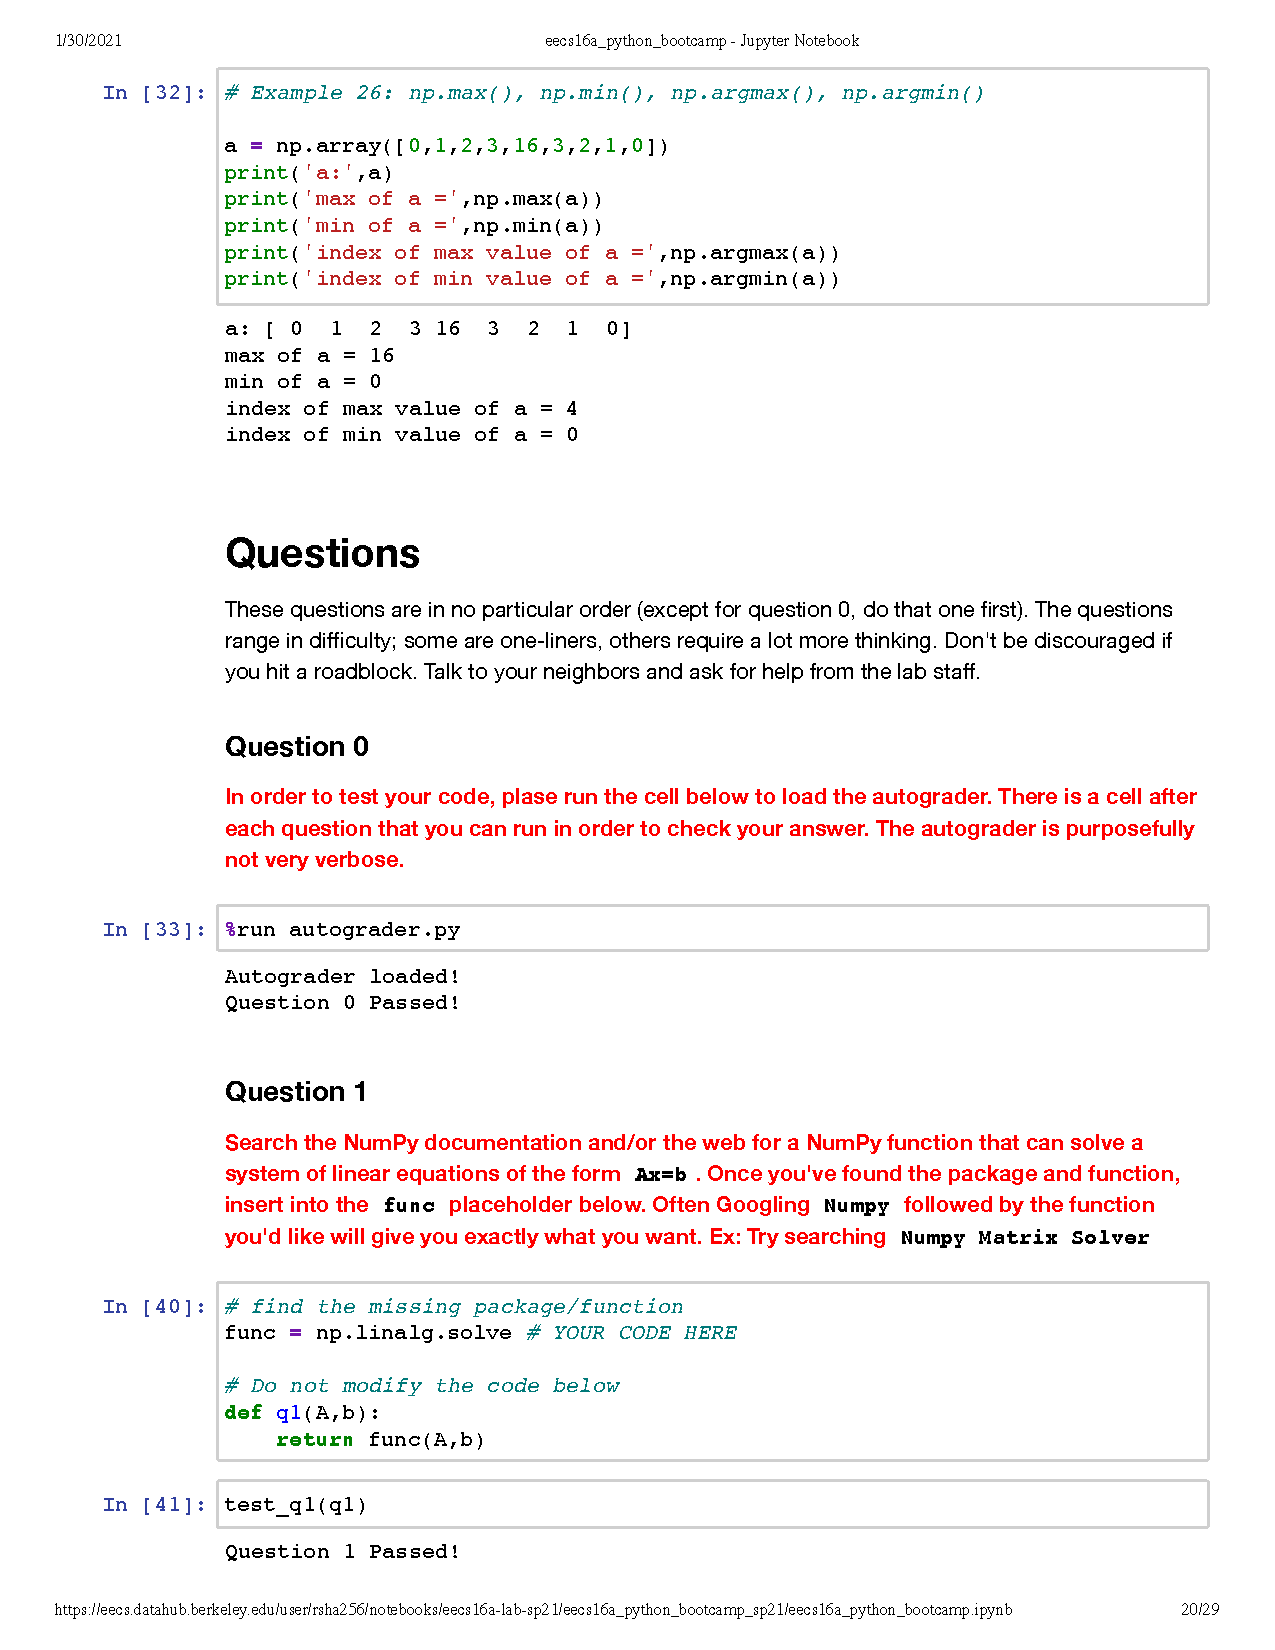
\includepdf[pages=-, noautoscale=true, scale=.8]{my_ipyntbk.pdf}

\newpage
\item $\textbf{Audio File Matching}$
	Many audio processing applications rely on representing audio files as vectors, referred to as audio signals.
	Every component of the vector determines the sound we hear at a given time. We can use inner products to determine if a particular audio clip is part of a longer song, similar to an application like Shazam. 
	
	Let us consider a very simplified model for an audio signal, $\vec x$. At each timestep $k$, the audio signal can be either $x[k] = -1$ or $x[k] = 1$.
\begin{enumerate}
    \item Say we want to compare two audio files of the same length N to decide how similar they are. First, consider two vectors that are exactly identical, namely $\vec x_1 = \begin{bmatrix} 1 & 1 & \cdots & 1 \end{bmatrix}^T$ and $\vec x_2 = \begin{bmatrix} 1 &  1 & \cdots & 1 \end{bmatrix}^T$. What is the inner product of these two vectors? What if $\vec x_1 = \begin{bmatrix} 1 & 1 & \cdots & 1 \end{bmatrix}^T$ but $\vec x_2$ oscillates between1 and -1? Assume that $N$, the length of the two vectors, is an even number.
    
    Use this to suggest a method for comparing the similarity between a generic pair of length-$N$ vectors.
	    \begin{Answer}
	        ...
	    \end{Answer}

	\item Next, suppose we want to find a short audio clip in a longer one. We might want to do this for an application like Shazam, which is able to identify a song from a short clip. Consider the vector of length 8, $\vec x = \begin{bmatrix} -1 & 1 & 1 & -1 & 1 & 1 & -1 & 1\end{bmatrix}^T$.
    
    We want to find the short segment $\vec y := \begin{bmatrix} y[0] & y[1] & y[2] \end{bmatrix}^T = \begin{bmatrix} 1 & 1 & -1\end{bmatrix}^T$ in the longer vector. To do this, perform the linear cross correlation between these two finite length sequences and identify at what shift(s) the linear cross correlation is maximized. Apply the same technique to identify what shift(s) gives the best match for $\vec y = \begin{bmatrix} 1 & 1 & 1 \end{bmatrix}^T$.
    
    (If you wish, you may use iPython to do this part of the question, but you do not have to.)
	    \begin{Answer}
	        ...
	    \end{Answer}

    \newpage
    \item Now suppose our audio vector is represented using integers beyond simply just 1 and -1. Find the short audio clip $\vec y = \begin{bmatrix} 1 & 2 & 3 \end{bmatrix}^T$ in the song given by $\vec x = \begin{bmatrix} 1 & 2 & 3 & 1 & 2 & 2 & 3 & 10 \end{bmatrix}^T$. Where do you expect to see the peak in the correlation of the two signals? Is the peak where you want it to be, 
    
    i.e. does it pull out the clip of the song that you intended? Why?
    (If you wish, you may use iPython to do this part of the question, but you do not have to.)
	    \begin{Answer}
	        ...
	    \end{Answer}

    \item Let us think about how to get around the issue in the previous part. We applied cross-correlation to compare segments of $\vec x$ of length 3 (which is the length of $\vec y$) with $\vec y$. Instead of directly taking the cross correlation, we want to normalize each inner product computed at each shift by the magnitudes of both segments, i.e. we want to consider $\frac{\l\vec x_k, \vec y\r}{||\vec x_k|| ||\vec y||}$, where $\vec x_k$ is the length 3 segment starting from the $k$-th index of $\vec x$. This is referred to as normalized cross correlation. Using this procedure, now which segment matches the short audio clip best?
	    \begin{Answer}
	        ...
	    \end{Answer}
	    
\end{enumerate}

	      			      		   
\newpage
\item $\textbf{Homework Process and Study Group}$

Who did you work with on this homework? List names and student ID’s. (In case you met people at homework party or in office hours, you can also just describe the group.) How did you work on this homework? If you worked in your study group, explain what role each student played for the meetings this week.
	      			      		        
\begin{Answer}
		      				      			            
\end{Answer}
\end{enumerate}
	      			      		
	      			      		
\newpage

\end{document}
